\chapter{Current issues in the FDI literature}
\label{chap:literature_issues}

At first glance, it makes sense to assume that all countries would be eager to
receive FDI. Indeed, FDI brings capital, creates jobs, contributes tax revenue,
and promises technological spillover to the local economy. Consider the impact
of an Intel's factory on Vietnam's economy. In 2006, Intel chose Saigon Hi-tech
Park in Ho Chi Minh City as the site for its \$1 billion chip testing and
assembly facility, its largest in the world. In 2016, Intel Products Vietnam
(IPV) employed 4000 workers at full capacity, exported \$3.45 billion worth of
goods (or 18.2\% of Vietnam's electronics export), and generated more than \$100
million for Vietnam's GDP in tax payment, salary, and profit. In addition, IPV
developed an engineering education program in partnership with Arizona State
University and local universities, educating thousands of young Vietnamese
engineers. As a result, IPV's workers were vastly more productive. While IPV's
workforce only constituted 5\% of all workers, its export value amounted to 72\%
of all export at the Saigon Hi-tech Park. Intel's decision to choose Ho Chi Minh
City over other candidate sites, including Chennai (India), Bangkok (Thailand),
and Dalian (China), was also a significant marketing boost to Vietnam's image as
a destination capable of high-tech manufacturing. Following Intel, many other
MNCs opened high-tech facilities in Vietnam, including Samsung's three factories
(in 2009, 2013, and 2014), Nokia/Microsoft (2012), and LG (2013)
\citep{Dinh2016, UNCTAD2008}.

In addition, economists have also developed long-standing theories about the
benefits of FDI. According to \citet{Findlay1978}, FDI plays a key
role in economic growth by upgrading the local economy's technological
capability. As well-known from neoclassical growth theory, diminishing returns
to capital will at one point stop capital from accumulating further, preventing
long-run economic growth from being driven by capital accumulation alone
\citep{Solow1956}. FDI counteracts this dynamic by helping local workers and
suppliers upgrade their productivity, either via training or demonstration.

Economic theories and captivating anecdotes notwithstanding, there are reasons
to believe that FDI benefits are not a given and that countries' preference for
FDI is not homogeneous. Indeed, cross-country studies show little evidence of
FDI inflow having a systematic and positive effect on growth
\citep{Nair-Reichert2001, Carkovic2002} or poverty reduction \citep{Gohou2012}.
Instead, the benefits of FDI is highly conditional on the absorptive capacity of
the host economies, i.e. its level of human capital, technological
sophistication, or financial market development \citep{Durham2004,
  Nunnenkamp2004, Fu2008, Willem2004}. Therefore, whether a country welcomes FDI
may depend on its economic conditions. Furthermore, while the capital brought
and jobs created by FDI may be good for the overall economy, its distributional
effects cut across constituencies, creating political cleavage across both
sectoral and geographical divides \citep{Chintrakarn2012, Goldberg2007,
  Nunnenkamp2007}. There are winners and losers for each FDI project, and their
relative political strength may determine the country's attitude towards FDI.

For these reasons, we should reject the standard assumption in the FDI
literature that countries universally want to attract FDI. In this chapter, I
take apart this assumption, providing qualitative evidence of countries having a
restrictive attitude towards FDI (Section~\ref{sec:demand_for_FDI}), and a
strategic targeting of specific kinds of FDI
(Section~\ref{sec:demand_for_FDI_types}). Finally, I discuss the limitation of
FDI flow data, the main dependent variable of the FDI literature
(Section~\ref{sec:measuring_mnc_activities}). Not only does FDI flow data not
map to political science concepts, its aggregated nature also prevents political
scientists from studying different types of FDI. The data limitation thus
reinforces the conceptual neglect of variation in countries' preference.
Fortunately, my two-sided matching model is able to deal with all of these
issues at the same time.

\section{Countries' demand for FDI}
\label{sec:demand_for_FDI}

\subsection{The untenable assumption of universal demand for FDI}

The IPE literature on the political determinants of FDI has largely focused on
what MNCs demand from countries. In this literature, politics matters, but only
in terms of what political factors make countries attractive to MNCs. As
\citet{Jensen2008b} states in the introduction of ``\textit{Nation-states and the
  Multinational Corporation}'':

\begin{quote}
  Which government policies prove beneficial to multinational corporations?
  Which political institutions provide multinational corporations with credible
  commitments to these market-friendly policies? These emerge as the central
  questions of this book.\footnote{Other scholars share the same line of
    inquiry, e.g.
  \citet{Ahlquist2006, Busse2007, Buthe2008, Li2003}.}
\end{quote}

In theorizing FDI inflow largely as a function of MNCs' preference, the FDI
literature implicitly assumes that countries are eager to receive as much FDI as
possible. On the contrary, a historical and comparative examination of FDI
policies makes it clear that countries have at best had a mixed attitude towards
foreign capital. As an example, consider the FDI policies of a rapidly
industrializing country, who within 30 years of intense globalization had
overtook incumbent industrial giants to become the factory of the world and the
largest recipient of FDI. I am writing, of course, about the US at the turn of
the 20\textsuperscript{th} century. From 1879 to 1909, the US transformed itself
from an economy dominated by agriculture (53\%) to one dominated by industry
(62\%). In 1914, it surpassed Britain's industrial output, producing more than
one third of the global output. During this period, the US was the most
popular destination for global capital and the world's greatest debtor nation
\citep[part II]{Wilkins1989}.

Despite its staunch advocacy for liberal FDI policies nowadays, the US had a
mixed attitude towards attitude when it was a net FDI recipient. While American
businesses were aware of the benefits, e.g. funding for risky ventures in mining
and railroad, complaints against FDI were equally common. Some grumbled that the
``tribute'' paid to foreign financiers were odious. Others in the railroad
industry felt that foreign management could not understand American problems and
might ruin the industry with demands for restructuring. Yet other protests
stemmed from a nationalistic belief that that ``our land'' should not be
controlled by European absentee owners. Such sentiments led to various state
legislation that, among other things, forbade nonresident alien ownership of
land, or tightened regulations around foreign financial institutions, including
banks, insurance companies, and mortgage lenders. Similarly, in 1913 the federal
government forbade foreign citizens from serving as directors of US national
banks, and only allowed them to buy share of US banks if they were willing to be
represented by US citizens on the board \citep[part II]{Wilkins1989}. Many of
these entry restrictions are still familiar tools of countries today.

A similarly restrictive attitude towards FDI characterized South Korea's
policies during its industrializing period. After almost half a century of
oppression under Japanese colonialism, South Korea was deeply averse to a large
foreign presence in their economy. This nationalistic impulse translated into a
host of restrictions on FDI entry and ownership. Throughout the 1960s and 1970s,
instead of keeping a small list of restricted sectors, Korea used a positive
list system that forbade FDI in all sectors except those explicitly allowed by
the government. Even in sectors that allowed FDI, majority foreign ownership was
also forbidden \citep{Thurbon2006}. Even as late as the 1980s, after mounting
internal pressure for a more liberal FDI policies, 50\% of all industries and
20\% of manufacturing industries were still closed to MNCs, and only 5\% of MNCs
in Korea were wholly owned by the foreign investor \citep{Chang2004}. On top of
these explicit restrictions, a FDI project must also be approved by numerous
agencies, including the Ministry of Trade and Industry, the Ministry of Science
and Technology, and the Ministry of Finance. The subsequent red tape and delay
further deterred MNCs from entering.\footnote{The arduous approval process for
  FDI projects was a deliberate policy choice by the Korean government and not
  the result of lacking state capacity. Indeed, as \citet{Evans1995} describes,
  Korea had a strong and autonomous state, capable of outlining and executing a
  developmental strategy for the country. Its FDI policies were an integral part
  of this strategy, as outlined in the Economic Planning Board (EPB)'s
  \textit{White Paper on Foreign Investment} \citep{EPB1981}. Korea's policy of
  meticulous vetting stands in stark contrast with recent efforts to fast track
  FDI projects (often called the ``one-stop shop'') promoted by international
  organizations, e.g. in Dominican Republic \citep{UNCTAD2016}, Nigeria
  \citep{UNCTAD-Nigeria2009}, and many others.} Instead of attracting FDI, Korea
relied much more on foreign debt for its capital need. As a result, from 1962 to
1983, FDI made up only 5.1\% of foreign capital in Korea while the rest was
debt (author's calculation based on data reported in \citet[92, Table
4.5]{Amsden1989}).

More importantly, countries are not just naively open or restrictive towards
FDI, but very strategic in formulating FDI policies that fit their political and
economic conditions. Therefore, if we make blanket assumption about countries'
demand for FDI instead of studying its variation, we overlook this strategic
component entirely. For example, consider the case of China, whose demand for
FDI has ebbed and flowed dramatically over time. Before, during, and after its
economic reform, China's attitude towards FDI swung from extreme hostility, to
red carpet treatment, and finally chilly co-existence. Indeed, prior to 1979,
there was virtually no foreign capital in China as Chinese leaders
self-congratulated on their nationalistic self-sufficiency. They even turned
down foreign aid from the International Red Cross for the 1976 Tangshang
earthquake, announcing that such disasters ``teach the value of self-reliance
and hard struggle'' \citep{Butterfield1976}. However, when the disastrous result
of central planning and the Cultural Revolution became apparent, especially in
stark contrast with the shining achievements of its neighboring Asian tigers,
China committed to Deng Xiaoping's ``open door policy'' in 1979. With the
promulgation of the ``Law on Chinese Foreign Equity Joint Ventures,'' the flood
gate opened for foreign capital \citep{Wei1996}. Throughout the reform period,
China's FDI policies continuously grew friendlier. In 1986, after Deng
Xiaoping's famous Southern tour to shore up support for reform, China moved from
``permitting'' to ``encouraging'' FDI, allowed wholly owned foreign enterprises,
and adopted a negative list approach that accepted FDI in all sectors unless
specifically banned. Finally, after China joined the WTO in 2001, China
abolished various performance requirements (e.g. export ratio, local content,
technology transfers, etc.) previously imposed on foreign firms
\citep{Long2005}.

During this reform period, China did not just allowed FDI---it even
discriminated against the domestic sector in favor of foreign firms. While
Chinese leaders continued to view the domestic sector with suspicion, they had
no problem with foreign firms, whose main goal was to make money and not to
raise political trouble \citep{Gallagher2002}. As a result, China created a
dualist legal regime that much better protected foreign firms than domestic
ones. For example, China created a 1979 law and a 1982 constitutional amendment
not to expropriate from foreign enterprises. There was no such guarantee for the
domestic sector. Compared to domestic firms, foreign businesses also seemed to
enjoy fewer audits, more favorable judgment during labor dispute, and more
assistance from the government \citep{Huang2003, Huang2011}. During the early
years of reform, FDI firms enjoyed such large benefits that even state-owned
enterprises (SOEs) were eager to form joint venture with them
\citep[59]{Gu1997}.

However, as China shifted its growth strategy to nurturing its domestic sector
into a world class competitor, its attitude towards FDI and domestic firms
reversed. In 2010, some European firms started grumbling about unfair
treatments, especially in sectors where intellectual property was important,
while others remained happy with making good money. As an observer remarked,
``China still welcomes FDI, but \ldots it is becoming more insistent on setting
the terms,'' including favoritism towards domestic firms for government
contracts, higher tax rate, or a limit on the number of non-Chinese staff
\citep{Grant2010}. By 2016, the accusations of discrimination against foreign
firms had become mainstream. A former deputy trade representative for the US
complained that foreign insurers had to apply for one license at a time, taking
six to eight months total. In contrast, despite claims of equal treatment from
the government, Chinese rivals could submit their whole package and got approved
much quicker. In its annual business climate survey, the American Chamber of
Commerce in China reported that, between 2015 and 2017, 75\% to 81\% of
businesses felt that they were less welcome than before
\citep[39]{AmCham2018}.\footnote{The business climate survey first asked this
  question in 2015.} James McGregor, former bureau chief of the Wall Street
Journal, chairman of AmCham China, and a business executive who lived in
China for more than two decades, observed \citep{Wu2016}:

\begin{quote}
  For foreign companies in China, right now is perhaps the most distressing and
  unhappy time that I have seen. \ldots They feel that the best days for foreign
  companies in China are reaching an end.
\end{quote}

In sum, the prevailing assumption in the FDI literature that all countries are
eager for FDI is untenable. Many countries, including those that eventually
become staunch supporters of liberalizing FDI policies, have held restrictive
policies on FDI when they were net recipient of FDI. More importantly, countries
also show a dynamic demand for FDI, adapting their policies to meet their
political and economic goals.

Unfortunately, the two common empirical approaches in the FDI literature
strongly rely on this assumption. In the first approach, researchers build a
regression model with FDI inflow as the dependent variable and a political
factor as the independent variable of interest. In this model, it is impossible
to interpret the political factor as an attraction to MNC or as a motivator of
countries' demand for FDI. Consider \citet{Jensen2005}'s finding that federalism
is positively associated with FDI inflow. The authors interpret this correlation
as federalism constraining the whim of the central government, increasing policy
stability, and thus making the country attractive to MNCs. However, the
alternative explanation is that local governments in a decentralized system
compete more intensely for FDI, driving up the FDI inflow. For example, as China
decentralized in the late 1980s and early 1990s, local governments gained the
authority to approve foreign investment up to a certain size, thus able to court
MNCs without asking the central government for permission.\footnote{Similar to
  China's broader economic reform, decentralization in China's FDI policies
  happened incrementally. In 1979, China first allowed FDI in four Special
  Economic Zones, i.e. Shenzhen, Zhuhai, Shantou (near Hong Kong), and Xiamen
  (near Taiwan). As the economic benefits of FDI became clear, provinces started
  clamoring for the ability to attract FDI themselves. Therefore, in 1984, China
  allowed 14 coastal cities to approve FDI projects, and in the early 1990s,
  allowed inland regions to do the same. \citet{Gallagher2002} and
  \citet{Shirk1993} discuss how the coalition for decentralization expanded over
  this period, and \citet{Coase2012} provides a historical account of China's
  economic reform more broadly.} In addition, local governments could keep all
revenue in excess of a quota pre-negotiated with the central government, further
motivating them to bring in MNCs as a lucrative source of tax revenue. Having
both the authority and the incentive to attract MNCs, Chinese local governments
engaged in an intense competition for MNCs. While there were only
117 development zones in 1991, the number exploded to 2700 in 1992, of which
only 95 were initiated by central ministries \citep{Montinola1995}. Far from
\citet{Jensen2005}'s argument, China's federalism did not increase FDI inflow by
producing a static policy environment that MNCs like. On the contrary,
federalism incentivized Chinese local governments to demand FDI, fostering local
policy experiments that were anything but stable.\footnote{A very similar
  account of decentralization causing provincial demand and competition for FDI
  happened in Vietnam as well \citep{Malesky2004c}.}

In the second approach, researchers estimate MNCs' preference using the discrete
choice model. The dependent variable is the MNC's choice of a location over all
the other options, and the independent variable of interest is a characteristic
of the location \citep{Arauzo-Carod2010}. In the discrete choice model, the
assumption is that all locations are available for the MNC to pick and choose,
effectively ruling out the possibility that the host country can decline the
MNC's investment proposal. Such an assumption is unfounded. For example, in
2007, Da Nang, a central province of Vietnam known for its public governance
quality, turned down \$2.5 billion dollars from a Taiwanese-Japanese steel
factory and a Japanese paper pulp factory for environmental concerns
\citep{HDung2007}. In 2014, even during tough times, when Da Nang's and
Vietnam's FDI inflow was merely half of the previous year, its attitude towards
FDI remained selective. According to Mr. Lam Quang Minh, Director of Da Nang's
investment promotion agency, the province declined a \$200-million Hong Kong
textile factory and a 30-hectare Korean dyeing facility, even when ``these
[refusals] have contributed to Da Nang's lackluster FDI attraction recently''
\citep{HaiChau2015}. While Da Nang is the most well-known, other Vietnamese
provinces have also refused large FDI projects that use too much land, exploit
natural resources, or cause environmental degradation \citep{QuocHung2015}.

\subsection{Current approaches to estimate countries' demand for FDI}

Unlike the FDI literature, the broader field of IPE has recognized that
countries' preference remains an important force even in a globalized era.
Indeed, despite early pessimism about countries engaging in a race to the bottom
to attract footloose global capital, scholars have shown substantial variation
in countries' trade, welfare, environmental, and fiscal policies
\citep{Drezner2001}. The FDI literature has lagged behind in this aspect.

Recognizing this gap, \citet{Pinto2013} and \citet{Pandya2016} recently broke
ground in this area. Similar to the rich IPE literature in international trade,
these studies argue that countries' demand for FDI varies according to FDI's
distributive effect on their domestic constituencies \citep{Broz2001,
  Milner2005a}. In this theoretical framework, labor supports FDI because
foreign firms bring capital that increases the demand for labor and raises
productivity, both of which lead to higher wage. On the other hand, domestic
firms oppose FDI because foreign firms compete for local labor, inputs, and
markets. Both \citet{Pinto2013} and \citet{Pandya2016} formulate their theories
as a variant of this labor-vs-business tension, which surfaces in the former
work as left-vs-right governments, and in the latter as
democratic-vs-authoritarian regimes.

While these pioneering works have enriched our understanding of the relationship
between politics and FDI, their empirical approaches do not satisfactorily
measure countries' demand for FDI, leaving their theoretical arguments untested.

Consider \citet{Pinto2013}'s approach. The author controls for economic and
institutional factors that affect FDI flow into a country, then claims that
what's left in the residual is the country's demand for
FDI.\footnote{Specifically, the estimation of FDI openness involves two steps.
  First, the author runs a gravity model explaining bilateral FDI flows,
  estimating the intercept as the host country-year fixed effect. Second, this
  fixed effect is then regressed on several economic and endowment factors of
  that country-year (i.e. GDP, GDP per capita, average school years, arable
  land). The residual in the second stage is considered the country's ``FDI
  openness'' in that year.} For this approach to be valid, every economic,
institutional, and endowment factors that affect FDI flow has to be controlled
for, leaving only the country's demand in the error term. This claim is much
stronger than the common assumption of exogenous error, which is valid as long
as the omitted factors are uncorrelated with the independent variable of
interest. Framed substantively, since the residual is likely to contain more
than just the country's demand for FDI, if we observe an abnormally high level
of FDI, we do not know whether it is because the country welcomes FDI or because
MNCs find something attractive in the country.\footnote{In addition, this
  approach requires data on bilateral FDI flow, ideally disaggregated by
  sectors. Therefore, this approach is limited to OECD countries only
  \citep{Pinto2008}. During the period the authors study, 1980-2000, OECD
  countries account for 95\% of global FDI outflow and 90\% of inflow. However,
  since then the role of the developed world in global FDI has declined sharply,
  reducing to 60.8\% of outflow and 40.6\% of inflow in 2014
  \citep{UNCTAD2015}.}

In contrast to \citet{Pinto2013}'s statistical approach, \citet{Pandya2014,
  Pandya2016} attempts to find a proxy for countries' demand for FDI. The author
uses the US Overseas Business Reports to construct the number of
industries that have foreign ownership restrictions or face investment
screening. The advantages of this measurement are its ease of interpretation and
its availability for many countries. However, two problems remain. First, adding
up the raw count of restricted industries is not appropriate because industries
are not the same. For example, given the reach of the banking sector into all
corners of the economy, a country's opening up its financial industry indicates
much more FDI-friendliness than, say, allowing foreign furniture makers to set
up shops. Since the theoretical argument is driven by FDI's distributive effect,
we must not ignore the varying impact of FDI across sectoral constituencies.

Second, according to the coding rule, an industry is coded as free if there is
no mention of restriction. However, when there is little FDI, US Overseas
Business Reports may find it not worth mentioning and does not report the
restrictions. Therefore, ``zero restriction'' in the dataset can either mean
that a country is very closed or very open to FDI. This concern is not
hypothetical. Figure \ref{fig:china_fdi_restriction} shows that, following the
coding of the US Overseas Business Reports, China seemed 100\% open to FDI up
until 1986 when it started imposing restrictions. The reality is the opposite.
Prior to 1986, only limited FDI was allowed as joint-venture in Special Economic
Zones (SEZ). The year of 1986 was, in fact, the first time China allowed any
wholly owned FDI outside of SEZs.

\begin{figure}[tbp] \centering
  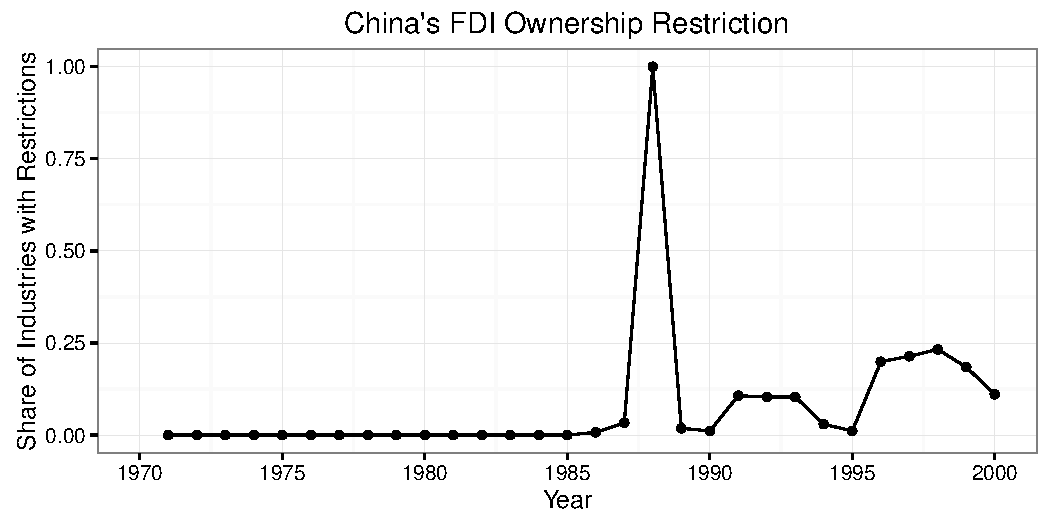
\includegraphics[width=0.8\textwidth,keepaspectratio]{china_fdi_restriction}
  \caption[China's FDI ownership restriction.]{China's FDI ownership
    restriction, as coded in \citet{Pandya2010}. Prior to 1986, FDI in China was
    limited to few experimental Special Economic Zones, and thus not mentioned
    in US Investment Reports. The sharp spike in 1988 also does not seem to
    correspond to any actual change in policy, and likely another artifact of
    reporting. (See \citet{Zebregs2002} for a historical overview of China's FDI
    policy.)}
  \label{fig:china_fdi_restriction}
\end{figure}

The two-sided matching model circumvents these thorny measurement issues by
modeling countries' demand for FDI directly. Intuitively, if we observe that a
country welcomes certain firms to invest but not others, we can compare the
characteristics of the invited and the uninvited firms to infer that country's
preference for FDI.

\section{Countries' preference for types of FDI}
\label{sec:demand_for_FDI_types}

\subsection{The untenable assumption that countries treat all types of FDI are
  the same}

In the literature of political determinants of FDI, the most common dependent
variable is aggregate FDI inflow in a country-year.\footnote{Only the OECD has a
  dataset of FDI broken down by sectors, limited to 34 OECD member countries.
  Source: OECD International direct investment database.} While relying on this
dependent variable, researchers focus almost exclusively on the quantity
of FDI, treating all FDI as one homogeneous flow of capital. Such emphasis on
aggregate FDI quantity is likely just an artifact of the data limitation. Indeed,
country case studies show that countries have a rich tapestry of policies
targeting specific types of FDI, tailored to their own political and economic
conditions. Below, I discuss such targeting strategy of Korea, Taiwan, and Costa
Rica.

\textit{Korea}. Not only did Korea restrict FDI entry in general, they also
aggressively screened FDI proposals for desirable qualities. To ensure that FDI
served its developmental strategy, Korea let its developmental pilot bureau, the
Economic Planning Board (EPB), take charge of FDI policies. The EPB displayed a
sophisticated understanding of the costs and benefits of FDI. Its 1981
\textit{White Paper on Foreign Investment} recognized that FDI could benefit
Korea by bringing capital, job creation, potential technological upgrading, and
hard currency. At the same time, it cautioned that MNCs might engage in transfer
pricing, demand distortionary import-export protection, crowd out domestic
investors, delay domestic technological capability, and even exert political
influence on the government \citep[50-64, quoted in
\citet{Chang2004}]{EPB1981}.\footnote{It is remarkable that the White Paper
  touched on all arguments in academic circles, showing that the Korean
  government paid close attention to the effects of FDI.} Therefore, in pursuit
of Korea's ``national ownership'' growth strategy, the EPB heavily restricted
MNCs that sought access to the domestic market, especially in labor-intensive
sectors where the government believed there were domestic alternatives. On the
other hand, the EPB prioritized FDI projects that were export oriented or more
technologically advanced than Korean firms. The EPB especially coveted MNCs that
would improve the capabilities of Korean producers, e.g. by procuring from local
suppliers, transferring technologies to local partners, providing access to
foreign markets, even divesting the foreign-held equities to the Korean
counterpart after a specified period. Indeed, of \$1.3 billion in FDI that
flowed into Korea between 1962 and 1983, Korean partners repurchased \$263.5
million (20\%) by 1983, after they had gained the production knowledge
\citep[135]{Mardon1990}. Korea accomplished this feat partly by providing
subsidized loans to the domestic partners, but more importantly by being willing
to turn down MNCs that did not agree to the stringent terms. According to
\citet{Mardon1990}'s survey of 45 foreign investors, such requirements were the
norm to enter the Korean economy. In 1986, 38\% of foreign firms committed to
exporting a fixed amount, 80\% to transferring technology, 36\% to supplying raw
materials not available domestically, and 28\% to helping Korean producers
access untapped export markets.

\textit{Taiwan.} In the 1960s, capital-strapped Taiwan was permissive in
admitting FDI, not screening for high-quality projects. However, in the 1970s,
Taiwan became increasingly selective, evaluating investment proposals based on
``how much they open new markets, build new exports, transfer technology,
intensify input-output links, make Taiwan more valuable to multinationals as a
foreign investment site and as a source for important components, and enhance
Taiwan's international political support'' \citep[151]{Wade1990}. Taiwan was so
firm on their targeting strategy that, in 1963, they overrode local firms'
objection and allowed Singer Sewing Machine Company, arguing that this FDI
foreign project could provide much needed currency and improve the quality of
local parts. Indeed, after one year, Singer did so much in terms of transferring
technology and boosting exports that local producers changed their mind
\citep{Ranis1985}. Another example of Taiwan's commitment to their FDI targeting
strategy was how they selected the MNC to build a polyethylene plant for the
domestic market. Taiwan insisted that the MNC exported any surplus over domestic
needs, refrained from building any other facilities in the downstream sector
(lest they compete with Taiwanese firms), and agreed to sell half of their
equities to Taiwanese partners after five years.\footnote{The deal was not all
  sticks and no carrots. In exchange for the stringent terms, Taiwan offered a
  five-year tax holiday, restrictions on import of competing products,
  guaranteed supply of an important chemical input, and unlimited repatriation
  of profits.} These demands were not cheap talk. During the negotiation
process, Taiwan rejected a Japanese investor who refused to comply to these
terms, and pick National Distiller, an US firm that fit Taiwan's target
\citep[151]{Wade1990}.

Interestingly, with China's shadow constantly loomed large, Taiwan's FDI
strategy depended not only on its economic strategy but at times also on its
security need. In the late 1970s, when the relationship between the US and
mainland China thawed, jeopardizing Taiwan's survival, the government made a big
effort to attract famous US MNCs. In contrast to the ruthless terms of other FDI
deals, Taiwan's invitation to GM to invest was extremely generous, providing
import protections and allowing GM to pull out at any time if it deemed that the
government failed to adequately protect its market power. However, by 1982, when
the US derecognition of Taiwan turned out not to be apocalyptic, GM's
affiliation with the US was no longer such a desirable. Taiwan thus
withdrew its concessions, prompting GM to leave \citep{Noble1987}.

\textit{Costa Rica.} With the spread of WTO membership, free trade agreements,
and investment treaties, the aggressive FDI policies adopted by the Korean and
Taiwanese governments may no longer be available to countries
today.\footnote{The WTO's Agreement on Trade-Related Investment Measures (TRIMS)
  forbids the practice of local content requirement, which forces MNCs to
  purchase local products, impeding free trade. Several Bilateral Investment
  Treaties (BITs) and Free Trade Agreements (FTAs) further ban other performance
  requirements, such as technology transfer. In addition, most investment
  agreements include obligations on ``national treatment,'' ensuring that
  countries cannot treat foreign firms worse than domestic firms. Under the
  current policy regime, many of Korea's and Taiwan's FDI policies are no longer
  legal and have become less frequently used, albeit not completely abandoned,
  by other countries \citep{Cosbey2015}.} However, while the discriminatory
tactics are gone, countries' desire to target types of FDI remains, manifesting
less often as requirements and more as encouragement. Costa Rica's success in
targeting high-tech FDI was a prime example. In mid-1990s, as other Central
American competitors entered the apparel export industry after a bout of civil
wars, Costa Rica was determined to diversify away from the textile industry,
breaking away from the cycle of competing on wage and offering unsustainable
fiscal incentives. Setting its sight on technologically advanced industries,
Costa Rica actively courted MNCs in these sectors. Leading the effort was Costa
Rica Investment Promotion Agency (CINDE), a private organization whose lobbying
efforts were initially financed by USAID and politically supported by an
alliance of bankers, exporters, and economists \citep{Clark1995}. CINDE had
typical investment promotion functions, including image building, investment
facilitation and aftercare, investment targeting, and policy advocacy for a
better business environment. However, CINDE provided these services only to
targeted industries, i.e. advanced manufacturing, life science, and services.
For MNCs in these sectors, CINDE systematically addressed investors' concern,
assisted with the establishment process, held regular check-in sessions, and
advocated for their interests pro-actively. In contrast, when a non-targeted
firm raised a complaint with CINDE, it simply relayed the message to relevant
government agencies \citep{OECD2013}.

Costa Rica's extraordinary effort to target desirable FDI was evident during the
negotiation to attract Intel's \$300 million assembly facility. At the time,
Intel's shortlist of candidate sites include Brazil, Chile, Indonesia, Thailand,
Mexico, and Costa Rica. The two finalists, Costa Rica and Mexico, reflecting
Intel's goal to diversify its geographical risk by expanding into Latin America.
Seizing this opportunity, CINDE coordinated Ministry of Energy and Environment,
Transportation, Finance, Science, and Technology to promptly address Intel's
concern, setting up electricity substations, a dedicated call center,
more frequent flights, consulates in the Philippines and Malaysia, and many
more. Even President Figueres also took a personal interest in the project,
traveling to Intel headquarters in Arizona to demonstrate Costa Rica's
commitment. The endeavor proved Costa Rica's strong preference for high-tech FDI
like Intel. In the end, Intel's decision to open the facility in Costa Rica was
a ``stamp of approval'' for Costa Rica's targeting strategy
\citep[511]{Mortimore2004}.\footnote{See \citet{Spar1998} for a detailed account
  of how Costa Rica beat out much more advantaged competitors like Mexico and
  Brazil, convincing Intel to invest despite initial reservations about Costa
  Rica's size and level of development.}

\subsection{Current approaches to estimate countries' preference for types of
  FDI}

Despite qualitative evidence of countries targeting specific types of FDI, two
data limitations prevent researchers from studying this variation in countries'
preference. First, FDI flow data typically does not disaggregate into types of
FDI. Studying FDI flow to the OECD, \citet{Alfaro2007} attempt to get around
this problem by using Germany's sectoral skill intensity as the proxy for the
FDI quality in a certain sector. However, to do so is to assume that 1)
Germany's sectoral variation is the same as everyone else's in the OECD, and 2)
there is little variation in skill intensity within a sector. Both assumptions
are untenable, especially since the authors divide all manufacturing industries
into only two categories: low skill and high skill.

Second, even if we can differentiate types of FDI, it remains an open question
how to estimate countries' preference for them. \citet{Alfaro2007} use
information from websites of investment promotion agencies (IPA) and survey
response as a proxy for their countries' preference---if an IPA lists an
industry as a ``target industry,'' the authors say that the country wants to
attract that type of FDI. While this approach seems reasonable at first glance,
Figure~\ref{fig:IPA_target_industries} shows that there is little variation in
what IPAs claim to be their target industries. Because investment promotion is
mainly a marketing and aspirational exercise, almost everyone claims that they
target manufacturing, advanced manufacturing, and infrastructure. In addition,
if we use IPAs as a proxy for countries' preferences, we must also take into
account the fact that countries which decide to establish an IPA may not be the
same as those who do not. Both of these issues are not addressed by
\citet{Alfaro2007}, and we are still in need of a way to estimate countries'
preference for different types of FDI.

\begin{figure}[tbp] \centering
  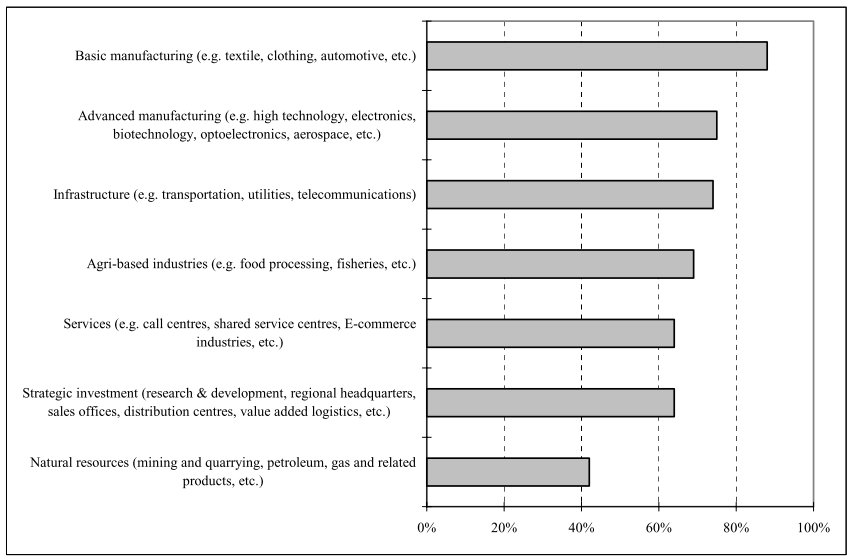
\includegraphics[width=\textwidth,keepaspectratio]{../figure/IPA_target_industries}
  \caption[Target industries by IPAs around the world.]{Target industries by
    IPAs around the world. Because of the image building aspect of investment
    promotion, almost all IPAs say that they want to attract ``manufacturing,''
    ``advanced manufacturing,'' and ``infrastructure.'' Therefore, using what is
    listed as investment priorities may not be a reliable way to measure
    countries' preference for FDI. Source: \citet{UNCTAD2001}.}
  \label{fig:IPA_target_industries}
\end{figure}

To address these challenges, we can use FDI firm-level data, which provides
information on not only a firm's sector but also its operational
characteristics, such as research and development (R\&D) expenditure or export
intensity. These measures are firm-specific and get closer to what countries are
looking for in FDI projects. Then, using firms' characteristics as covariates in
the two-sided matching model, I will be able to estimate countries' preferences
for these traits.

\section{Measuring MNCs' activities}
\label{sec:measuring_mnc_activities}

As \citet{Kerner2014} argues, the IPE literature on FDI is a bit of a misnomer.
Political scientists are rarely interested in FDI \textit{per se}---rather, they
are interested in the activities of MNCs, which in turn, affect other important
issues such as nation-state autonomy \citep{Mosley2005}, economic development
\citep{Moran1998}, labor standards \citep{Mosley2007}, and environmental
policies \citep{Prakash2007}. However, while the theory involves MNCs as the
central actor in the causal mechanism, the empirics often uses FDI flow as the
variable of interest. These two concepts---the level of MNCs' affiliate
activities in a country and FDI inflow into a country---are not the same.

Consider the definition of FDI from UNCTAD, the main producer of FDI data widely
used by researchers:

\begin{quote} FDI has three components: equity capital, reinvested earnings and
  intra-company loans.
  \begin{itemize}
  \item Equity capital, i.e. the foreign investor’s purchase of shares of an
    enterprise [in the host country].
  \item Reinvested earnings, i.e. the foreign investor’s share \ldots of
    earnings not distributed as dividends by affiliates, or earnings not
    remitted to the foreign investor.
  \item Intra-company loans between direct investors and affiliate enterprises.
  \end{itemize} \citep[245]{UNCTAD2007}
\end{quote}

In essence, FDI data captures the amount of capital that crosses border. It is a
poor proxy for the scale of MNCs' activities in the host country because it
overlooks important components of MNCs' activities while including irrelevant
components that only matter for balance of payment statistics
\citep{Beugelsdijk2010}.

Consider the argument that FDI is the driver for the diffusion of labor
standards across countries. \citet{Mosley2007} theorize that FDI can have this
effect through three channels. First, MNCs may pressure the host government for
better rule of law and social programs. For MNCs to be able to effectively exert
this pressure, they must prove themselves valuable to the government by
providing jobs or tax revenue. Both of these factors are tenuously related to
the amount of foreign capital inside the host country. Indeed, an MNC can employ
thousands of employees, pay millions in tax, but show up as a net 0 on FDI flow
data because of profit repatriation or intra-company loans.\footnote{The issue
  of intra-company loans is particularly fraught with issues because companies
  very frequently use intra-company loans to get out of paying tax in a country.
  These loans will be recorded on the book as a massive outflow, even though the
  MNC still has a large presence on the ground.} The scale of MNCs' operation is
further understated because FDI statistics does not take into account capital
raised locally. Also not included is the superior productivity of MNCs, which
acts as an important multiplier when translating the amount of capital to the
amount of output.

Second, scholars argue that MNCs may bring along best practices for workers'
rights and spread it to local firms. If this spillover effect happens via
competition, i.e. MNCs providing better working condition and forcing local
firms to compete, then MNCs must employ a lot of labor for this effect to be
noticeable. If the spillover happens via demonstration, then MNCs must form a
lot of linkages with local firms, as suppliers and buyers, for the diffusion of
norms to happen. Both the size of the labor force and the type of linkages with
the local economy are not captured by FDI flow statistics.

Third, scholars argue that MNCs may invest in higher wages, better benefits, or
more training. Once again, for this effect to be noticeable, the MNC's industry,
size of labor force, and investment in productivity matter a lot more than how
much capital it brings in and out of the country. In addition, non-equity
transactions between the parent company and the subsidiary, such as transfer of
knowledge, technology, and management practices, are not counted in FDI flow
statistics, thus excluding another component that is much more
important to labor quality than the amount of capital.\footnote{These issues are
  not isolated to studies of FDI and labor standards, but are common to the
  whole IPE literature of the effect of FDI on policy convergence, such as
  environmental policies \citep{Prakash2007}.}

This mismatch between theory and empirics may also be a reason behind the
unsettled debate on the effect of FDI on poverty reduction. Scholars have
theorized that FDI can lead to economic development through three channels:
cheaper goods, technology transfer, and tax revenue. Once again, the causal
variable in the second and third channels is the scale and the type of MNCs'
activities in the host country, not necessarily the amount of capital crossing
the border. Indeed, productivity spillover is highly conditional on the
technological capability of the MNC and whether it forms thick linkages with
local suppliers. The effect of FDI via tax revenue is also fraught with issues,
as MNCs frequently use intra-company transactions to artificially reduce book
profit and get out of paying tax \citep{Malesky2015c}.\footnote{This practice is
  called ``transfer pricing,'' and can include tactics such as charging for
  internal intellectual properties and services whose price can be set
  arbitrarily by the firm} Since FDI flow statistics do not record these
intra-company transactions, it is not surprising that researchers reach the
confusing conclusion that FDI does not generate tax revenue.

What about studies that use FDI as the dependent variable, and are thus perhaps
interested in the flow of capital in and of itself?\footnote{Arguably, political
  scientists are not interested in the flow of capital in and of itself.
  Instead, the flow of global capital matters because of its implications for
  development, state autonomy, and other effects on policy. The discussion above
  has shown how problematic it is to study these effect of FDI using FDI flow
  data.} The vast majority of these studies on the determinants of FDI flow rely
on the ``obsolescing bargain'' model. Originally developed by
\citet{Vernon1971}, the model is so named because the bargaining dynamics
between the MNC and the host government changes over time. Initially, the mobile
MNC can threaten to invest elsewhere and thus has the stronger bargaining power.
However, after the MNC has committed fixed capital on the ground, the host
government gets the upper hand. Indeed, knowing that it is costly for the MNC to
uproot its increasingly large and immobile operation, the host government can
unilaterally alter the original bargain, most egregiously by expropriating the
MNC's asset and profit, but more often via ``creeping expropriation,'' e.g.
increased tax or tougher regulation \citep{Li2009a}. Political economists argue
that MNCs are acutely aware of the ``obsolescing bargain,'' and thus prefer to
invest in countries whose governments can make a credible commitment that they
will not alter the original deal. This argument translates into a large
literature claiming that MNCs prefer countries with democratic accountability
\citep{Jensen2003}, a federal system \citep{Jensen2005}, membership in
international trade agreements \citep{Buthe2008}, less political risk
\citep{Graham2010}, or more veto points \citep{Choi2008}.

The linchpin of this argument is the assumption that FDI capital is illiquid and
cannot be quickly removed from the host country at will. This assumption is not
fully warranted. According to the US Bureau of Economic Analysis (BEA)'s 2004
survey, 43\% of US MNCs' balance sheet comprises of liquid assets that can be
liquidated within one year under normal operating situations. Among the 57\% of
the balance sheet that is illiquid, 24\% is ``other non-current assets,'' which
include non-tangible assets like brand names, trademarks, and patents---some of
which are not expected to be liquidated but can be easily removed from host
countries. Only another 24\% of the balance sheet is physical capital, i.e.
Plant, Property, and Equipment (PPE), which cannot be easily moved and match
most closely to what we have in mind as the ``illiquid capital'' in the
obsolescing bargain model \citep[113]{Kerner2014a}. Since FDI flow data does not
distinguish between liquid and illiquid capital, it is suspect to use FDI flow
data to test the ``obsolescing bargain'' argument, calling into questions the
entire literature on the political determinants of FDI.

Besides the conceptual mismatch between FDI flow and MNCs' activities, from a
statistical standpoint, this measurement error may also be a contributing factor
to why there is little consensus in the FDI literature. Even if the measurement
error is random, it will inflate the standard error of our estimate when FDI is
the dependent variable, and bias our estimate towards 0 when FDI is the
independent variable. These effects may explain \citet{Jensen2012}'s surprising
finding that lower corporate tax rate does not lead to more FDI flow, or the
mixed empirical evidence for the relationship between FDI and development
\citep[108]{Mold2004}.

Even more worryingly, the measurement error is unlikely to be
random.\footnote{See \citet{Gallop2017} for a recent and more comprehensive
  discussion of measurement error in political science research.} For example,
the amount of locally raised capital---an important source of capital for MNCs
yet not captured in FDI flow data---is likely to correlate with how developed
the local capital market is or how wildly the exchange rate fluctuates.
Similarly, repatriated earnings, which does not necessarily indicate reduced
MNCs' activities but is recorded as an outflow in FDI flow data, is likely to
correlate with the tax rate of not only the host country but also other tax
havens that the MNC may have an affiliate in.

To deal with this measurement error problem, scholars have attempted to use
measurements other than FDI flow. Given that political scientists are often
interested in MNCs' activities, recent work emphasizes using MNCs' operational
data directly. These firm-level datasets allow researchers to measure directly
the quantities of interest. For example, re-visiting \citet{Li2009a}'s
hypothesis that democracies are more attractive to MNCs, \citet{Kerner2014} uses
data on US MNCs' fixed capital expenditure to more precisely test the
relationship between democratic institutions and FDI \textit{illiquid} capital,
not just FDI in general. The author finds that there is no relationship between
democratic institutions and FDI flow, but there is a positive relationship
between democracy and MNCs' fixed capital expenditure, confirming the
theoretical expectation. Similarly, when \citet{Jensen2008a} re-examines whether
MNCs favor democratic regimes because they pose less political risk, the author
avoids using FDI flow and relies on price data of political risk insurance
agencies instead.\footnote{Scholars in other areas of IPE are also paying more
  attention to the issue of measurement error and the mismatch between empirics
  and theory, e.g. \citet{Karcher2013}.}

\section{Next steps}

In sum, the current FDI literature would benefit from studying countries'
demand for FDI, distinguishing types of FDI, and using firm-level
operational data instead of aggregate FDI flow statistics. While the theoretical
needs are clear and firm-level data has become more abundant in recent years,
political scientists have not developed a model to estimate this data structure
appropriately.\footnote{Examples of firm-level data include the US Bureau of
  Economic Analysis (BEA)'s survey of all US firms abroad, Tokyo Keizai's
  Overseas Japanese companies database (\textit{Kaigai Sinshutsu Kigyou
    Souran}), World Bank's Enterprise Survey, and Orbis database of companies
  worldwide.}

Very often, given the data structure of a set of firms interacting with a set of
countries, scholars resort to a dyadic-based analysis perhaps due to its being a
familiar tool. In such analysis, the unit of observation is a firm-country dyad,
and the model used is typically OLS regression. Each dyad is assumed to be
independent of each other, and any bias caused by interdependency is fixed via
post-estimation procedures, such as clustered standard errors \citep{Dorff2013}.
Unfortunately, this dyadic approach is patently inappropriate to analyze MNCs'
investment location. Indeed, once an MNC chooses to open a subsidiary in a
country, that subsidiary is by definition not located in another. Therefore, the
values of firm-country dyads deterministically constrain one another and cannot
be modeled as independent draws from a common distribution.\footnote{As a recent
  example, \citet{Arel-Bundock2017} uses Orbis, a global dataset of firms, to
  study the location decision of MNCs. The author uses random forest, a
  non-parametric machine learning approach, to predict whether an investment
  materializes for each of MNC-country dyad. However, because the predictors in
  the random forest model are dyad-specific, this approach cannot model
  interactions between dyads. In addition, since random forest does not produce
  interpretable coefficients, this black-box approach prevents us from
  understanding the preference of actors, how these preference are correlated
  with other characteristics, and how they may evolve over time.}

The two-sided matching model can simultaneously address all of these three
issues in the literature. This approach models the matching process explicitly,
thus taking into account the dependency across dyads. The matching process is
made up of actors maximizing their utility functions---therefore, we gain direct
insight into what countries and MNCs value the most. Finally, the model uses
firm-level operational data, circumventing the measurement error problem of
aggregate FDI flow statistics. In the next chapter, I describe in details how
the two-sided matching model is set up and estimated.

%%% Local Variables:
%%% mode: latex
%%% TeX-master: "AnhLe_dissertation.tex"
%%% End:
